\documentclass[10pt,A4]{article}	
\usepackage[utf8]{inputenc}

%----------------------------------------------------------------------------------------
%	LOGIC
%----------------------------------------------------------------------------------------

% provides \isempty test
\usepackage{xstring, xifthen}

%----------------------------------------------------------------------------------------
%	FONT BASICS
%----------------------------------------------------------------------------------------

\usepackage[default]{raleway}

% set font default
\renewcommand*\familydefault{\sfdefault} 	
\usepackage[T1]{fontenc}

%----------------------------------------------------------------------------------------
%	PAGE LAYOUT  DEFINITIONS
%----------------------------------------------------------------------------------------

% page outer frames (debug-only)
% \usepackage{showframe}	

% we use paracol to display breakable two columns
\usepackage{paracol}

\usepackage[a4paper]{geometry}
\geometry{top=1cm, bottom=1cm, left=0.5cm, right=0.5cm}

\usepackage{fancyhdr}
\pagestyle{empty}

% space between header and content
% \setlength{\headheight}{0pt}

% indentation is zero
\setlength{\parindent}{0mm}

%----------------------------------------------------------------------------------------
%	TABLE /ARRAY DEFINITIONS
%---------------------------------------------------------------------------------------- 

% extended aligning of tabular cells
\usepackage{array}

% custom column right-align with fixed width
% use like p{size} but via x{size}
\newcolumntype{x}[1]{%
>{\raggedleft\hspace{0pt}}p{#1}}%

%----------------------------------------------------------------------------------------
%	GRAPHICS DEFINITIONS
%---------------------------------------------------------------------------------------- 

%for header image
\usepackage{graphicx}

%for drawing graphics		
\usepackage{tikz}				
\usetikzlibrary{shapes, backgrounds, mindmap, trees}
	
%----------------------------------------------------------------------------------------
%	GLOBAL VARIBLES
%----------------------------------------------------------------------------------------

%----------------------------------------------------------------------------------------
%	Color DEFINITIONS
%---------------------------------------------------------------------------------------- 
\usepackage{transparent}
\usepackage{color}

% primary color
\definecolor{maincol}{RGB}{ 225, 0, 0 }

% accent color, secondary
% \definecolor{accentcol}{RGB}{ 250, 150, 10 }

% dark color
\definecolor{darkcol}{RGB}{ 70, 70, 70 }

% light color
\definecolor{lightcol}{RGB}{245,245,245}

%----------------------------------------------------------------------------------------
%   Profile
%----------------------------------------------------------------------------------------

\newcommand{\gfullname}{Nguyen Hoang Nam}
\newcommand{\gaddress}{2F 14 Street, District 7, HCM}
\newcommand{\gphone}{+84 90 236 59 38}
\newcommand{\gmail}{nguyenhoangnam.dev@gmail.com}
\newcommand{\ggithub}{Nguyen-Hoang-Nam}

%----------------------------------------------------------------------------------------
%	UTILS
%----------------------------------------------------------------------------------------

% returns minipage width minus two times \fboxsep
% to keep padding included in width calculations
% can also be used for other boxes / environments
\newcommand{\mpwidth}{\linewidth-\fboxsep-\fboxsep}

%----------------------------------------------------------------------------------------
%	FONT AWESOME ICONS
%----------------------------------------------------------------------------------------

\usepackage{fontawesome}

% use to vertically center content
% credits to: http://tex.stackexchange.com/questions/7219/how-to-vertically-center-two-images-next-to-each-other
\newcommand{\vcenteredinclude}[1]{\begingroup
\setbox0=\hbox{\includegraphics{#1}}
\parbox{\wd0}{\box0}\endgroup}

% use to vertically center content
% credits to: http://tex.stackexchange.com/questions/7219/how-to-vertically-center-two-images-next-to-each-other
\newcommand*{\vcenteredhbox}[1]{
    \begingroup
        \setbox0=\hbox{#1}\parbox{\wd0}{\box0}
    \endgroup
}

% icon shortcut
\newcommand{\icon}[3] { 							
	\makebox(#2, #2){\textcolor{maincol}{\csname fa#1\endcsname}}
}	

% icon with text shortcut
\newcommand{\icontext}[4]{ 						
	\vcenteredhbox{\icon{#1}{#2}{#3}}  \hspace{2pt}  \parbox{0.9\mpwidth}{\textcolor{#4}{#3}}
}

% icon with website url
\newcommand{\iconhref}[5]{ 						
    \vcenteredhbox{\icon{#1}{#2}{#5}}  \hspace{2pt} \href{#4}{\textcolor{#5}{#3}}
}

%============================================================================%
%
%	CV COMMANDS
%
%============================================================================%

%----------------------------------------------------------------------------------------
%	 CV LIST
%----------------------------------------------------------------------------------------

% renders a standard latex list but abstracts away the environment definition (begin/end)
\newcommand{\cvlist}[1] {
	\begin{itemize}{#1}\end{itemize}
}

%----------------------------------------------------------------------------------------
%	 CV TEXT
%----------------------------------------------------------------------------------------

% base class to wrap any text based stuff here. Renders like a paragraph.
% Allows complex commands to be passed, too.
% param 1: *any
\newcommand{\cvtext}[1] {
	\begin{tabular*}{1\mpwidth}{p{0.98\mpwidth}}
		\parbox{1\mpwidth}{#1}
	\end{tabular*}
}

%----------------------------------------------------------------------------------------
%	CV SECTION
%----------------------------------------------------------------------------------------

% Renders a a CV section headline with a nice underline in main color.
% param 1: section title
\newcommand{\cvsection}[1] {
	\vspace{4pt}
	\cvtext{
		\textbf{\Large{\textcolor{darkcol}{\uppercase{#1}}}}\\[-4pt]
		\textcolor{maincol}{ \rule{0.1\textwidth}{2pt} } \\
	}
}

%----------------------------------------------------------------------------------------
%	META SKILL
%----------------------------------------------------------------------------------------

% Renders a progress-bar to indicate a certain skill in percent.
% param 1: name of the skill / tech / etc.
% param 2: level (for example in years)
% param 3: description of skill
\newcommand{\cvskill}[3] {
	\begin{tabular*}{1\mpwidth}{p{0.72\mpwidth}  r}
 		\textcolor{black}{\large{\textbf{#1}}} & \textcolor{maincol}{#2}\\[4pt]
	\end{tabular*}
  	
  	\hspace{4pt}
  	\vspace{8pt}
  	\parbox{0.9\mpwidth}{#3}\\[2pt]
  	
  	\vspace{8pt}
}


%----------------------------------------------------------------------------------------
%	 CV EVENT
%----------------------------------------------------------------------------------------

% Renders a table and a paragraph (cvtext) wrapped in a parbox (to ensure minimum content
% is glued together when a pagebreak appears).
% Additional Information can be passed in text or list form (or other environments).
% the work you did
% param 1: time-frame i.e. Sep 14 - Jan 15 etc.
% param 2:	 event name (job position etc.)
% param 3: Customer, Employer, Industry
% param 4: Short description
\newcommand{\cvevent}[4] {
	
	% we wrap this part in a parbox, so title and description are not separated on a pagebreak
	% if you need more control on page breaks, remove the parbox
	\parbox{\mpwidth}{
		\begin{tabular*}{1\mpwidth}{p{0.20\mpwidth}  l}
	 		{#1} & \large{\textbf{#2}} \\[2pt]
			& \textbf{#3} \\
			& \parbox{0.75\mpwidth}{\small{#4}} \\
		\end{tabular*}\\[6pt]
	}
	\vspace{8pt}
}

\usepackage[hidelinks]{hyperref}

%============================================================================%
%
%
%
%	DOCUMENT CONTENT
%
%
%
%============================================================================%
\begin{document}
\columnratio{0.35}
\setlength{\columnsep}{0.5cm}
\setlength{\columnseprule}{4pt}
\colseprulecolor{lightcol}

\begin{paracol}{2}
\begin{leftcolumn}

%---------------------------------------------------------------------------------------
%	AVATAR
%---------------------------------------------------------------------------------------
\begin{center}
    \begin{tikzpicture}
        \clip circle (2.5cm); 
        \path (0,0) node{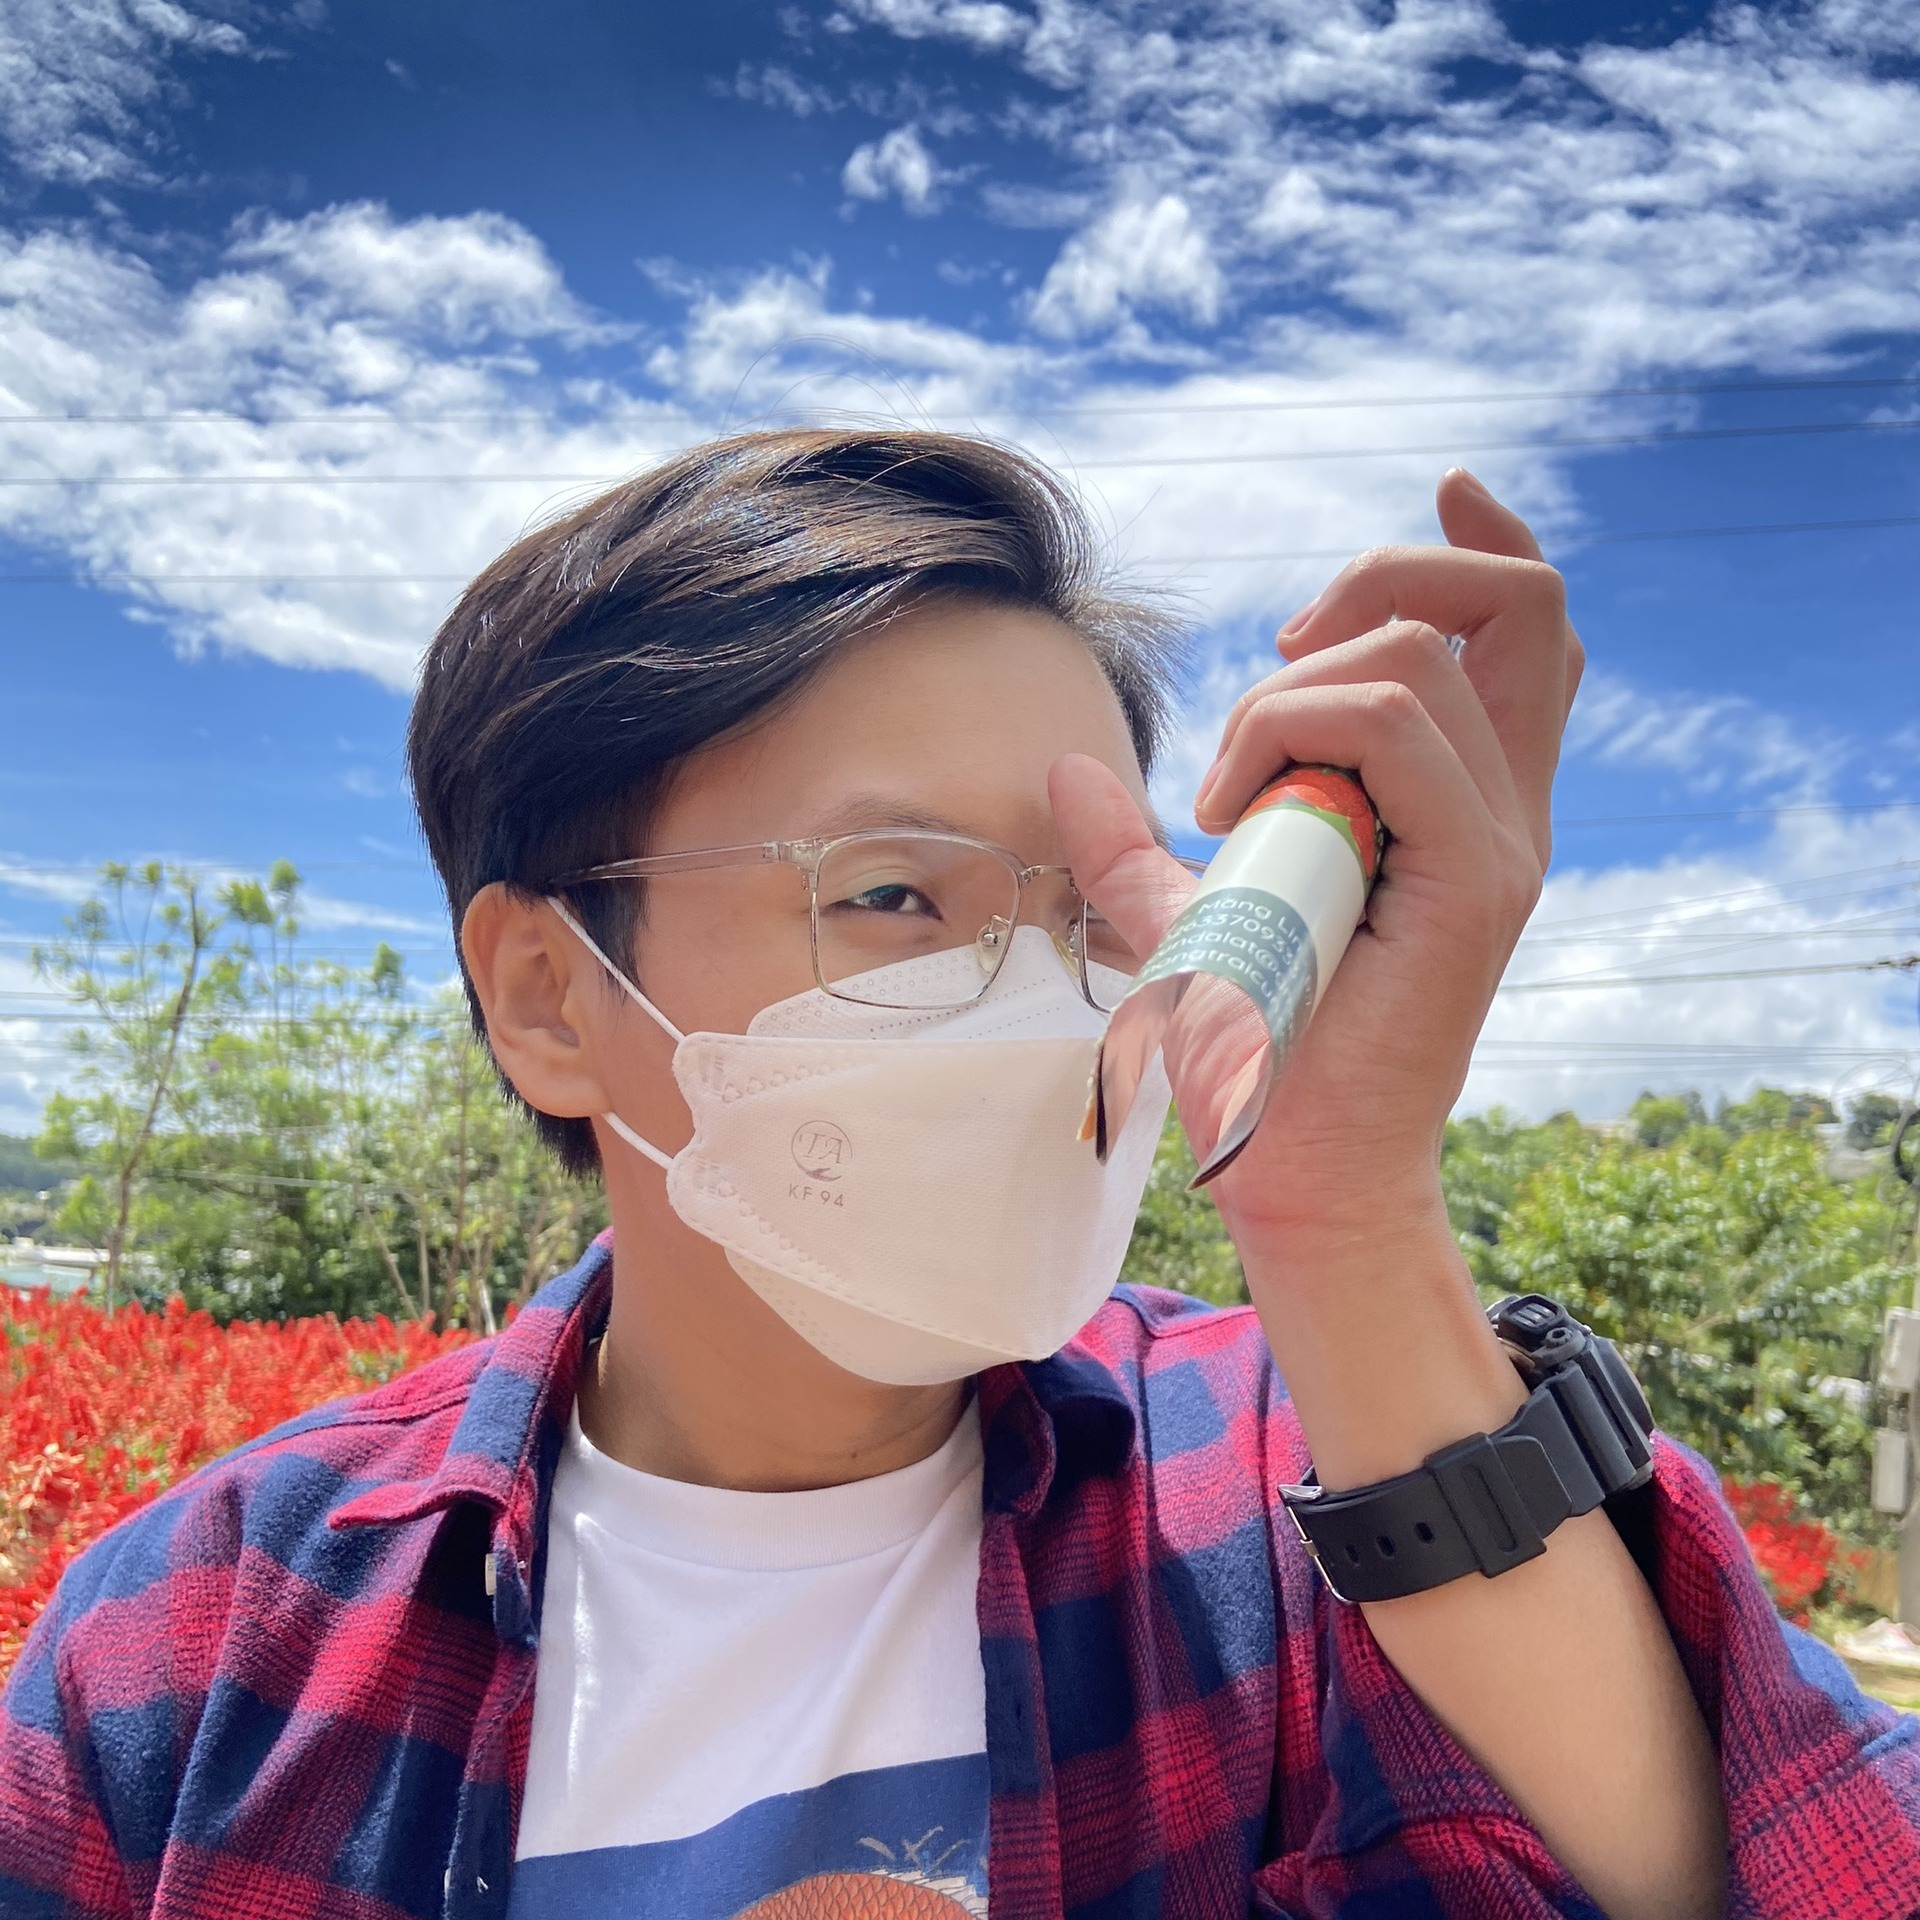
\includegraphics[width=5cm]{avatar.jpg}};
    \end{tikzpicture}
\end{center} 

%---------------------------------------------------------------------------------------
%	PROFILE
%----------------------------------------------------------------------------------------
\begin {center}
	\LARGE{ \textbf{ \uppercase{ \gfullname } } } \\[-10pt]
	\textcolor{red}{ \rule{0.1\textwidth}{1.25pt} } \\[10pt]
	\large{ Backend Developer with Three Years of Experience }
\end {center}

\icontext{MapMarker}{12}{\gaddress}{black}\\[6pt]
\icontext{Phone}{12}{\gphone}{black}\\[6pt]
\iconhref{Envelope}{12}{\gmail}{mailto:\gmail}{black}\\[6pt]
\iconhref{Github}{12}{\ggithub}{https://github.com/\ggithub}{black}\\[6pt]

%---------------------------------------------------------------------------------------
%	SKILLS
%----------------------------------------------------------------------------------------
\cvsection{SKILLS}

\cvskill{Elixir} {2+ years} {Phoenix, Ecto, Absinthe and Pow.}

\cvskill{Java} {2+ years} {Spring Boot, Spring Cloud, Eureka and API Gateway.}

\cvskill{JavaScript} {2+ years} {Express, React, Svelte and Solid.}

\cvskill{Go} {1+ years} {Gin and GRPC.}

\cvskill{Database} {2+ years} {Postgres, Mongo, Redis and Meilisearch.}

\cvskill{Cloud} {1+ years} {FCM, S3, SES, EC2, DynamoDB, and Lambda.}

\cvskill{Dev-Ops} {2+ years} {Ansible, Gitlab, Docker, Prometheus, Grafana and Github Action.}

\end{leftcolumn}
\begin{rightcolumn}

%---------------------------------------------------------------------------------------
%	WORK EXPERIENCE
%----------------------------------------------------------------------------------------
\cvsection{WORK EXPERIENCE}
    
\cvevent
    {2021}
    {BackEnd Microservices Developer}
    {FPT Telecom Company}
    {Our team is responsible for the development and maintenance of a chat service, as well as several other services. We utilize Spring Boot and Microservice architecture to deliver high-quality solutions for our large customer’s project.}
    
\cvevent
    {2022}
    {BackEnd Developer}
    {Beowulf Blockchain Company}
    {As a key member of the development team, I am responsible for the payment service within our travel system, which is a collaboration with Crystal Bay Company. This service is implemented using Elixir. In addition to this responsibility, I am also the lead developer for our event management system and flight booking service, both of which are also written in Elixir.}

%---------------------------------------------------------------------------------------
%	EDUCATION
%---------------------------------------------------------------------------------------
% \vfill\null
\cvsection{EDUCATION}

\cvevent
	{2018 - 2022}
	{Bachelor Degree of Computer Vision}
	{University of Science}
	{I possess a strong background of Computer Science, including algorithms, and OOP. I have experience designing databases and am currently expanding my knowledge in the field of Image Processing. My studies include Classification, Tracking, and Detection using advanced techniques such as CNNs, RNNs, GANs, and YOLO.}

%---------------------------------------------------------------------------------------
%	PROJECT
%---------------------------------------------------------------------------------------
% \vfill\null
\cvsection{PROJECTS}

\cvevent
	{9 - 2021}
	{OnCX}
	{FPT Telecom Company}
	{The platform designed to manage all aspects of an online business. This includes Call Center, Chat management, Comment management, CRM, and Voice bot integration. The core of the project was built using Spring Boot and a Microservices architecture to enable scalability and simplify the deployment process for our customers.}

\cvevent
	{5 - 2022}
	{Crystabaya}
	{Crystabaya Company}
	{The booking system that combines the features of other popular booking platforms with an NFT system. The platform is powered by the Phoenix framework and Postgresql, providing fast and reliable performance. Additionally, it is backed by MongoDB, Redis, and Meilisearch.}

\cvevent
	{9 - 2022}
	{Quickom Event}
	{Quickom Company}
	{The ticketing platform that helps organizations manage events in a crucial way. The platform includes features for managing tickets, promotions, and online events. The system was built using Phoenix and utilizes GraphQL for its API. It supports major payment methods such as Stripe, MOMO, and bank transfers.}

\cvevent
	{2 - 2022}
	{Crystabaya Flight}
	{Crystabaya Company}
	{The domestic flight booking platform that supports four major Vietnamese airlines: Vietnam Airlines, Vietjet, Bamboo Airways, and Vietravel. The system was built using Phoenix and employs multiple caching methods to improve the bottleneck problem of legacy Airline system.}

\end{rightcolumn}
\end{paracol}
\end{document}
